% Created by tikzDevice version 0.12.6 on 2026-09-17 23:39:55
% !TEX encoding = UTF-8 Unicode
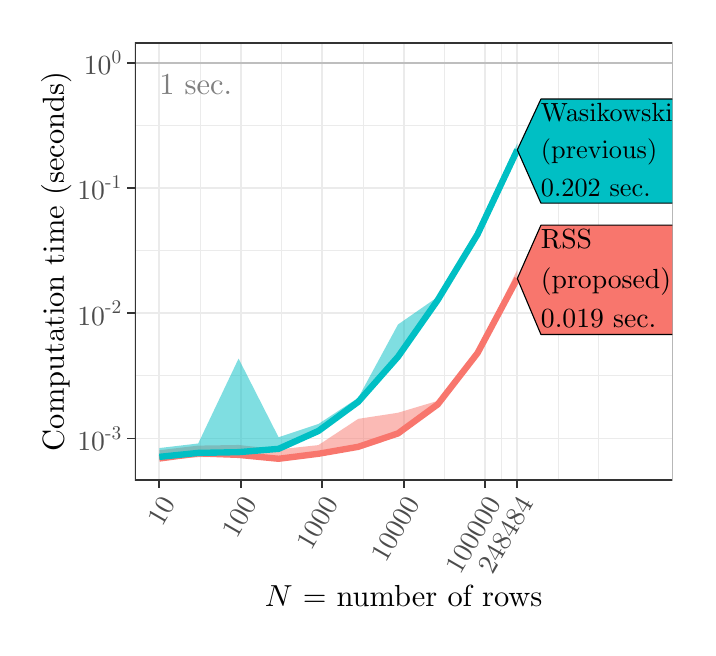
\begin{tikzpicture}[x=1pt,y=1pt]
\definecolor{fillColor}{RGB}{255,255,255}
\path[use as bounding box,fill=fillColor,fill opacity=0.00] (0,0) rectangle (238.49,216.81);
\begin{scope}
\path[clip] (  0.00,  0.00) rectangle (238.49,216.81);
\definecolor{drawColor}{RGB}{255,255,255}
\definecolor{fillColor}{RGB}{255,255,255}

\path[draw=drawColor,line width= 0.6pt,line join=round,line cap=round,fill=fillColor] (  0.00,  0.00) rectangle (238.49,216.81);
\end{scope}
\begin{scope}
\path[clip] ( 38.74, 53.30) rectangle (232.99,211.31);
\definecolor{fillColor}{RGB}{255,255,255}

\path[fill=fillColor] ( 38.74, 53.30) rectangle (232.99,211.31);
\definecolor{drawColor}{gray}{0.92}

\path[draw=drawColor,line width= 0.3pt,line join=round] ( 38.74, 91.00) --
	(232.99, 91.00);

\path[draw=drawColor,line width= 0.3pt,line join=round] ( 38.74,136.25) --
	(232.99,136.25);

\path[draw=drawColor,line width= 0.3pt,line join=round] ( 38.74,181.50) --
	(232.99,181.50);

\path[draw=drawColor,line width= 0.3pt,line join=round] ( 62.29, 53.30) --
	( 62.29,211.31);

\path[draw=drawColor,line width= 0.3pt,line join=round] ( 91.72, 53.30) --
	( 91.72,211.31);

\path[draw=drawColor,line width= 0.3pt,line join=round] (121.15, 53.30) --
	(121.15,211.31);

\path[draw=drawColor,line width= 0.3pt,line join=round] (150.58, 53.30) --
	(150.58,211.31);

\path[draw=drawColor,line width= 0.3pt,line join=round] (171.12, 53.30) --
	(171.12,211.31);

\path[draw=drawColor,line width= 0.3pt,line join=round] (191.65, 53.30) --
	(191.65,211.31);

\path[draw=drawColor,line width= 0.3pt,line join=round] (206.36, 53.30) --
	(206.36,211.31);

\path[draw=drawColor,line width= 0.6pt,line join=round] ( 38.74, 68.37) --
	(232.99, 68.37);

\path[draw=drawColor,line width= 0.6pt,line join=round] ( 38.74,113.62) --
	(232.99,113.62);

\path[draw=drawColor,line width= 0.6pt,line join=round] ( 38.74,158.87) --
	(232.99,158.87);

\path[draw=drawColor,line width= 0.6pt,line join=round] ( 38.74,204.13) --
	(232.99,204.13);

\path[draw=drawColor,line width= 0.6pt,line join=round] ( 47.57, 53.30) --
	( 47.57,211.31);

\path[draw=drawColor,line width= 0.6pt,line join=round] ( 77.00, 53.30) --
	( 77.00,211.31);

\path[draw=drawColor,line width= 0.6pt,line join=round] (106.44, 53.30) --
	(106.44,211.31);

\path[draw=drawColor,line width= 0.6pt,line join=round] (135.87, 53.30) --
	(135.87,211.31);

\path[draw=drawColor,line width= 0.6pt,line join=round] (165.30, 53.30) --
	(165.30,211.31);

\path[draw=drawColor,line width= 0.6pt,line join=round] (176.93, 53.30) --
	(176.93,211.31);
\definecolor{drawColor}{gray}{0.50}

\node[text=drawColor,anchor=base west,inner sep=0pt, outer sep=0pt, scale=  1.10] at ( 47.57,192.76) { 1 sec.};
\definecolor{drawColor}{RGB}{190,190,190}

\path[draw=drawColor,line width= 0.6pt,line join=round] ( 38.74,204.13) -- (232.99,204.13);
\definecolor{fillColor}{RGB}{248,118,109}

\path[fill=fillColor,fill opacity=0.50] ( 47.57, 64.11) --
	( 61.62, 65.79) --
	( 76.21, 66.02) --
	( 90.66, 64.41) --
	(105.06, 65.97) --
	(119.44, 75.45) --
	(133.81, 77.66) --
	(148.19, 81.96) --
	(162.56,100.11) --
	(176.93,129.36) --
	(176.93,125.91) --
	(162.56, 99.09) --
	(148.19, 80.23) --
	(133.81, 69.70) --
	(119.44, 64.54) --
	(105.06, 62.45) --
	( 90.66, 60.80) --
	( 76.21, 61.87) --
	( 61.62, 61.60) --
	( 47.57, 60.49) --
	cycle;

\path[] ( 47.57, 64.11) --
	( 61.62, 65.79) --
	( 76.21, 66.02) --
	( 90.66, 64.41) --
	(105.06, 65.97) --
	(119.44, 75.45) --
	(133.81, 77.66) --
	(148.19, 81.96) --
	(162.56,100.11) --
	(176.93,129.36);

\path[] (176.93,125.91) --
	(162.56, 99.09) --
	(148.19, 80.23) --
	(133.81, 69.70) --
	(119.44, 64.54) --
	(105.06, 62.45) --
	( 90.66, 60.80) --
	( 76.21, 61.87) --
	( 61.62, 61.60) --
	( 47.57, 60.49);
\definecolor{fillColor}{RGB}{0,191,196}

\path[fill=fillColor,fill opacity=0.50] ( 47.57, 64.90) --
	( 61.62, 66.56) --
	( 76.21, 97.23) --
	( 90.66, 68.81) --
	(105.06, 73.60) --
	(119.44, 83.05) --
	(133.81,109.54) --
	(148.19,119.52) --
	(162.56,142.63) --
	(176.93,175.08) --
	(176.93,172.30) --
	(162.56,141.77) --
	(148.19,117.89) --
	(133.81, 97.32) --
	(119.44, 81.30) --
	(105.06, 70.80) --
	( 90.66, 64.26) --
	( 76.21, 62.54) --
	( 61.62, 62.54) --
	( 47.57, 60.99) --
	cycle;

\path[] ( 47.57, 64.90) --
	( 61.62, 66.56) --
	( 76.21, 97.23) --
	( 90.66, 68.81) --
	(105.06, 73.60) --
	(119.44, 83.05) --
	(133.81,109.54) --
	(148.19,119.52) --
	(162.56,142.63) --
	(176.93,175.08);

\path[] (176.93,172.30) --
	(162.56,141.77) --
	(148.19,117.89) --
	(133.81, 97.32) --
	(119.44, 81.30) --
	(105.06, 70.80) --
	( 90.66, 64.26) --
	( 76.21, 62.54) --
	( 61.62, 62.54) --
	( 47.57, 60.99);
\definecolor{drawColor}{RGB}{248,118,109}

\path[draw=drawColor,line width= 2.3pt,line join=round] ( 47.57, 61.13) --
	( 61.62, 62.98) --
	( 76.21, 62.44) --
	( 90.66, 61.03) --
	(105.06, 62.84) --
	(119.44, 65.35) --
	(133.81, 70.19) --
	(148.19, 80.70) --
	(162.56, 99.23) --
	(176.93,126.17);
\definecolor{drawColor}{RGB}{0,191,196}

\path[draw=drawColor,line width= 2.3pt,line join=round] ( 47.57, 61.72) --
	( 61.62, 63.15) --
	( 76.21, 63.42) --
	( 90.66, 64.62) --
	(105.06, 71.08) --
	(119.44, 81.61) --
	(133.81, 97.89) --
	(148.19,118.42) --
	(162.56,142.13) --
	(176.93,172.67);
\end{scope}
\begin{scope}
\path[clip] ( 38.74, 53.30) rectangle (232.99,211.31);
\definecolor{drawColor}{RGB}{0,0,0}
\definecolor{fillColor}{RGB}{248,118,109}

\path[draw=drawColor,line width= 0.4pt,line join=round,line cap=round,fill=fillColor] (176.93,126.17) --
	(185.47,145.44) --
	(233.91,145.44) --
	(233.91,105.94) --
	(185.47,105.94) --
	cycle;
\definecolor{fillColor}{RGB}{0,191,196}

\path[draw=drawColor,line width= 0.4pt,line join=round,line cap=round,fill=fillColor] (176.93,172.67) --
	(185.47,191.02) --
	(234.41,191.02) --
	(234.41,153.40) --
	(185.47,153.40) --
	cycle;

\node[text=drawColor,anchor=base west,inner sep=0pt, outer sep=0pt, scale=  1.00] at (185.47,137.13) {RSS};

\node[text=drawColor,anchor=base west,inner sep=0pt, outer sep=0pt, scale=  1.00] at (185.47,122.73) {(proposed)};

\node[text=drawColor,anchor=base west,inner sep=0pt, outer sep=0pt, scale=  1.00] at (185.47,108.33) {0.019 sec.};

\node[text=drawColor,anchor=base west,inner sep=0pt, outer sep=0pt, scale=  0.95] at (185.47,183.07) {Wasikowski};

\node[text=drawColor,anchor=base west,inner sep=0pt, outer sep=0pt, scale=  0.95] at (185.47,169.41) {(previous)};

\node[text=drawColor,anchor=base west,inner sep=0pt, outer sep=0pt, scale=  0.95] at (185.47,155.75) {0.202 sec.};
\definecolor{drawColor}{gray}{0.20}

\path[draw=drawColor,line width= 0.6pt,line join=round,line cap=round] ( 38.74, 53.30) rectangle (232.99,211.31);
\end{scope}
\begin{scope}
\path[clip] (  0.00,  0.00) rectangle (238.49,216.81);
\definecolor{drawColor}{gray}{0.30}

\node[text=drawColor,anchor=base west,inner sep=0pt, outer sep=0pt, scale=  1.00] at ( 17.96, 64.08) {10};

\node[text=drawColor,anchor=base west,inner sep=0pt, outer sep=0pt, scale=  0.70] at ( 27.96, 68.17) {-};

\node[text=drawColor,anchor=base west,inner sep=0pt, outer sep=0pt, scale=  0.70] at ( 30.29, 68.17) {3};

\node[text=drawColor,anchor=base west,inner sep=0pt, outer sep=0pt, scale=  1.00] at ( 17.96,109.33) {10};

\node[text=drawColor,anchor=base west,inner sep=0pt, outer sep=0pt, scale=  0.70] at ( 27.96,113.42) {-};

\node[text=drawColor,anchor=base west,inner sep=0pt, outer sep=0pt, scale=  0.70] at ( 30.29,113.42) {2};

\node[text=drawColor,anchor=base west,inner sep=0pt, outer sep=0pt, scale=  1.00] at ( 17.96,154.58) {10};

\node[text=drawColor,anchor=base west,inner sep=0pt, outer sep=0pt, scale=  0.70] at ( 27.96,158.67) {-};

\node[text=drawColor,anchor=base west,inner sep=0pt, outer sep=0pt, scale=  0.70] at ( 30.29,158.67) {1};

\node[text=drawColor,anchor=base west,inner sep=0pt, outer sep=0pt, scale=  1.00] at ( 20.30,199.84) {10};

\node[text=drawColor,anchor=base west,inner sep=0pt, outer sep=0pt, scale=  0.70] at ( 30.29,203.93) {0};
\end{scope}
\begin{scope}
\path[clip] (  0.00,  0.00) rectangle (238.49,216.81);
\definecolor{drawColor}{gray}{0.20}

\path[draw=drawColor,line width= 0.6pt,line join=round] ( 35.99, 68.37) --
	( 38.74, 68.37);

\path[draw=drawColor,line width= 0.6pt,line join=round] ( 35.99,113.62) --
	( 38.74,113.62);

\path[draw=drawColor,line width= 0.6pt,line join=round] ( 35.99,158.87) --
	( 38.74,158.87);

\path[draw=drawColor,line width= 0.6pt,line join=round] ( 35.99,204.13) --
	( 38.74,204.13);
\end{scope}
\begin{scope}
\path[clip] (  0.00,  0.00) rectangle (238.49,216.81);
\definecolor{drawColor}{gray}{0.20}

\path[draw=drawColor,line width= 0.6pt,line join=round] ( 47.57, 50.55) --
	( 47.57, 53.30);

\path[draw=drawColor,line width= 0.6pt,line join=round] ( 77.00, 50.55) --
	( 77.00, 53.30);

\path[draw=drawColor,line width= 0.6pt,line join=round] (106.44, 50.55) --
	(106.44, 53.30);

\path[draw=drawColor,line width= 0.6pt,line join=round] (135.87, 50.55) --
	(135.87, 53.30);

\path[draw=drawColor,line width= 0.6pt,line join=round] (165.30, 50.55) --
	(165.30, 53.30);

\path[draw=drawColor,line width= 0.6pt,line join=round] (176.93, 50.55) --
	(176.93, 53.30);
\end{scope}
\begin{scope}
\path[clip] (  0.00,  0.00) rectangle (238.49,216.81);
\definecolor{drawColor}{gray}{0.30}

\node[text=drawColor,rotate= 60.00,anchor=base east,inner sep=0pt, outer sep=0pt, scale=  1.00] at ( 53.54, 44.91) {10};

\node[text=drawColor,rotate= 60.00,anchor=base east,inner sep=0pt, outer sep=0pt, scale=  1.00] at ( 82.97, 44.91) {100};

\node[text=drawColor,rotate= 60.00,anchor=base east,inner sep=0pt, outer sep=0pt, scale=  1.00] at (112.40, 44.91) {1000};

\node[text=drawColor,rotate= 60.00,anchor=base east,inner sep=0pt, outer sep=0pt, scale=  1.00] at (141.83, 44.91) {10000};

\node[text=drawColor,rotate= 60.00,anchor=base east,inner sep=0pt, outer sep=0pt, scale=  1.00] at (171.26, 44.91) {100000};

\node[text=drawColor,rotate= 60.00,anchor=base east,inner sep=0pt, outer sep=0pt, scale=  1.00] at (182.90, 44.91) {248484};
\end{scope}
\begin{scope}
\path[clip] (  0.00,  0.00) rectangle (238.49,216.81);
\definecolor{drawColor}{RGB}{0,0,0}

\node[text=drawColor,anchor=base,inner sep=0pt, outer sep=0pt, scale=  1.10] at (135.87,  7.64) {$N$ = number of rows};
\end{scope}
\begin{scope}
\path[clip] (  0.00,  0.00) rectangle (238.49,216.81);
\definecolor{drawColor}{RGB}{0,0,0}

\node[text=drawColor,rotate= 90.00,anchor=base,inner sep=0pt, outer sep=0pt, scale=  1.10] at ( 13.08,132.31) {Computation time (seconds)};
\end{scope}
\end{tikzpicture}
